%% Documentation for BOUT++ Drift instability test

\documentclass[12pt]{article}
\usepackage[nofoot]{geometry}
\usepackage{graphicx}
\usepackage{fancyhdr}
\usepackage{subfigure}

\usepackage{listings}
\usepackage{color}
\usepackage{textcomp}
\definecolor{listinggray}{gray}{0.9}
\definecolor{lbcolor}{rgb}{0.95,0.95,0.95}
\lstset{
	backgroundcolor=\color{lbcolor},
        language=C++,
	keywordstyle=\bfseries\ttfamily\color[rgb]{0,0,1},
	identifierstyle=\ttfamily,
	commentstyle=\color[rgb]{0.133,0.545,0.133},
	stringstyle=\ttfamily\color[rgb]{0.627,0.126,0.941},
	showstringspaces=false,
	basicstyle=\small,
	numberstyle=\footnotesize,
	numbers=left,
	stepnumber=1,
	numbersep=10pt,
	tabsize=2,
	breaklines=true,
	prebreak = \raisebox{0ex}[0ex][0ex]{\ensuremath{\hookleftarrow}},
	breakatwhitespace=false,
	aboveskip={1.5\baselineskip},
        columns=fixed,
        upquote=true,
        extendedchars=true,
        morekeywords={Field2D,Field3D,Vector2D,Vector3D,real,FieldGroup},
}

%% Modify margins
\addtolength{\oddsidemargin}{-.25in}
\addtolength{\evensidemargin}{-.25in}
\addtolength{\textwidth}{0.5in}
\addtolength{\textheight}{0.25in}
%% SET HEADERS AND FOOTERS

\pagestyle{fancy}
\fancyfoot{}
\renewcommand{\sectionmark}[1]{         % Lower case Section marker style
  \markright{\thesection.\ #1}}
\fancyhead[LE,RO]{\bfseries\thepage}    % Page number (boldface) in left on even
                                        % pages and right on odd pages 
\renewcommand{\headrulewidth}{0.3pt}

%% commands for boxes with important notes
\newlength{\notewidth}
\addtolength{\notewidth}{\textwidth}
\addtolength{\notewidth}{-3.\parindent}
\newcommand{\note}[1]{
\fbox{
\begin{minipage}{\notewidth}
{\bf NOTE}: #1
\end{minipage}
}}

\newcommand{\noun}[1]{\textsc{#1}}
\newcommand{\deriv}[2]{\ensuremath{\frac{\partial #1}{\partial #2}}}
\newcommand{\code}[1]{\texttt{#1}}
\newcommand{\file}[1]{\texttt{\bf #1}}
\newcommand{\pow}{\ensuremath{\wedge}}
\newcommand{\poweq}{\ensuremath{\wedge =} }

%\newcommand{\deriv}[2]{\ensuremath{\frac{\partial #1}{\partial #2}}}
\newcommand{\apar}{\ensuremath{A_{||}}}
\newcommand{\hthe}{\ensuremath{h_\theta}}
\newcommand{\Bp}{\ensuremath{B_\theta}}
\newcommand{\Bt}{\ensuremath{B_\zeta}}
\newcommand{\Vec}[1]{\ensuremath{\mathbf{#1}}}
\newcommand{\bvec}{\Vec{b}}
\newcommand{\kvec}{\Vec{\kappa}}
\newcommand{\bxk}{\bvec_0\times\kvec_0\cdot\nabla}
\newcommand{\Bvec}{\Vec{B}}
\newcommand{\Bbar}{\overline{B}}
\newcommand{\Lbar}{\overline{L}}
\newcommand{\Tbar}{\overline{T}}
\newcommand{\Jvec}{\Vec{J}}
\newcommand{\Jpar}{J_{||}}
\newcommand{\delp}{\nabla_\perp^2}
\newcommand{\Div}[1]{\ensuremath{\nabla\cdot #1 }}
\newcommand{\Curl}[1]{\ensuremath{\nabla\times #1 }}
\newcommand{\rbpsq}{\ensuremath{\left(R\Bp\right)^2}}

\begin{document}

\title{Resistive drift-wave instability test}
\author{B.Dudson, University of York \\
M.Umansky, LLNL}
\maketitle

\section{Introduction}

A drift-wave is a wave which exists in a plasma wherever there is a pressure
gradient \cite{hazeltine-2003}.
Without dissipation, fluctuations in density $n$ and electrostatic
potential $\phi$ are in phase
so there is no transport of plasma and the wave amplitude does not grow.
Dissipation, in this case resistivity, introduces a phase-shift
between $n$ and $\phi$ and hence transport of plasma and growth of the mode.
Since all that is required for radial transport is a pressure gradient
and some form of dissipation (in the absence of magnetic shear), this is often called the ``universal''
instability. 
Because the growth of the resistive drift-wave instability is sensitive to
phase shifts, this test checks how accurately this phase is simulated.

The equations solved are for the density $n$, and vorticity
$\omega = n_0\mathbf{b}\cdot\Curl{\mathbf{v}}$.
The simulation is electrostatic, and the zero electron mass approximation
is used to obtain the parallel current $j_{||}$. All quantities with a '$0$'
subscript are equilibrium and not evolved.
\begin{eqnarray*}
\deriv{n}{t} &=& -\mathbf{V}_E\cdot\nabla n_0 \\
\deriv{\omega}{t} &=& \frac{B_0^2}{m_i}\nabla_{||}j_{||} \\
\mathbf{V}_E &=& \frac{1}{B_0}\mathbf{b}_0\times\nabla_\perp\phi \\
\nabla_\perp^2\phi &=& \omega/n_0 \\
j_{||} &=& \sigma_{||}\left(T_0\partial_{||}n - n_0\partial_{||}\phi\right)
\end{eqnarray*}
The simulation domain is a cylindrical annulus with radius $R = 5.4$~m, radial width $6$~cm and constant
density scale-length $L_N = 4.5$~m. This is a 2D periodic simulation domain, but since perpendicular
wavenumber is fixed in a given simulation, the simulation is effectively 1D. Radial boundary conditions are
zero-gradient vorticity and density, and $\phi = 0$. 
Numerical methods used were $4^{th}$-order central differencing, and $3^{rd}$-order WENO for advection terms
on a 32x32 grid. A relative tolerance of \code{1.0e-7}, and absolute tolerance of \code{1.0e-12} were specified.

The analytic dispersion relation is $\left(\omega - \omega_*\right)i\sigma_{||} + \omega^2 = 0$, with
diamagnetic frequency $\omega_* = k T_{e0} / L_N$ \cite{umansky-2008-tests}.

\begin{figure}[htbp!]
\centering
\subfigure[Growth rate]{
  \label{fig:drift_imag}
  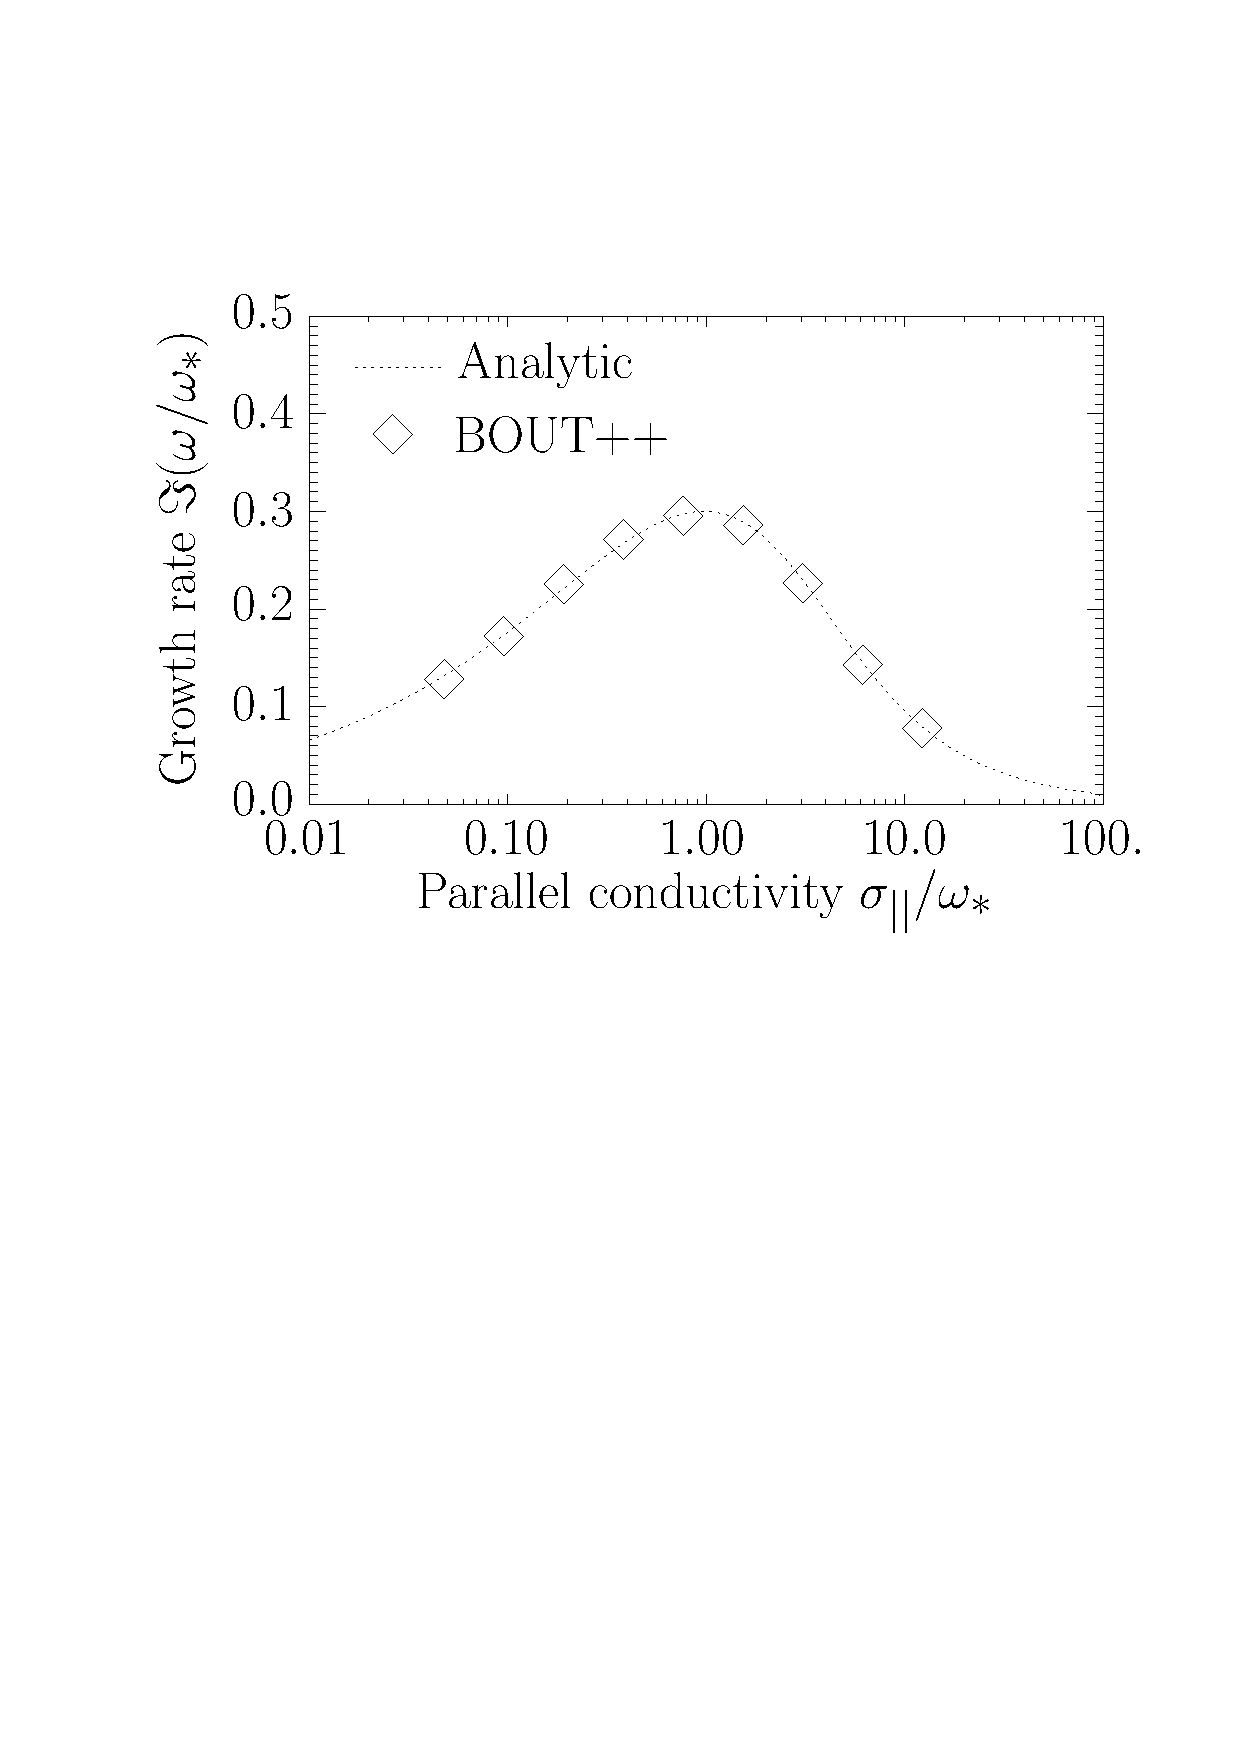
\includegraphics[scale=0.35]{drift_growth.pdf}
}
\subfigure[Real Frequency]{
  \label{fig:drift_real}
  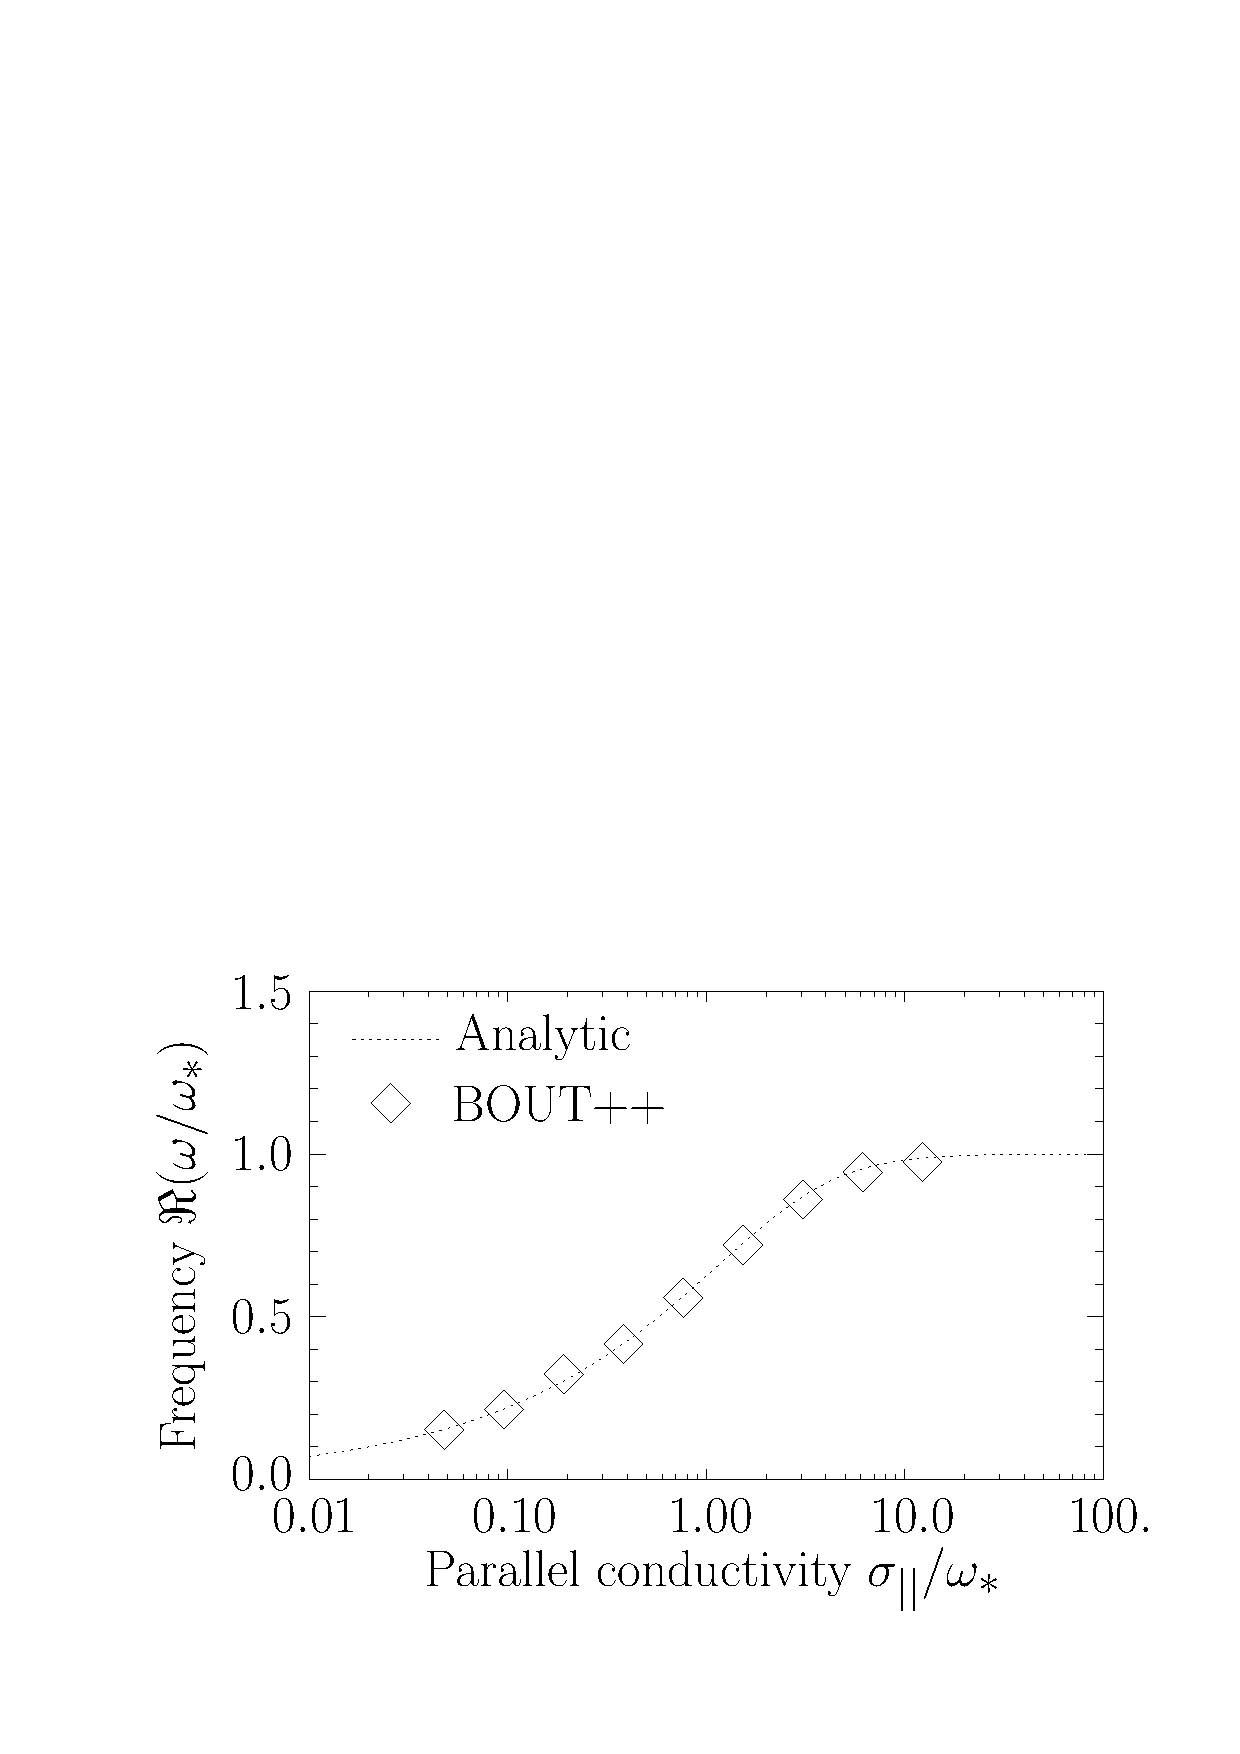
\includegraphics[scale=0.35]{drift_freq.pdf}
}
\end{figure}

\section{Input grid}

The input grid file \file{uedge.grd\_std.cdl} was created (by M.Umansky) for
BOUT-06, so the variables in the file were chosen for tokamak simulations. 
The following is a list of variables which are read in by this example code. For this drift instability
problem, most of these quantities are not used since the geometry is very simple.
\begin{itemize}
\item \code{nx} and \code{ny} : The size of the grid in X and Y; The size in the Z dimension is specified in the
options file (see next section). For this test, \code{nx = 5} which consists of 1 ``real'' point, and 2 boundary
cells either side.
\item \code{dpsi} : The X grid spacing in poloidal flux $\psi$
\item \code{dx}, \code{dy}. By default, BOUT++ uses these two for the X and Y grid spacing so reads them in
  at the beginning. Unfortunately, BOUT uses dpsi for the X spacing so this must be changed in this example code.
  \code{dy} is just a constant (in radians), as the Y spacing is given by \code{hthe}.
\item \code{Rxy[x,y]}, \code{Zxy[x,y]} : Major radius and height in meters of each grid point
\item \code{hthe[x,y]} : The poloidal distance between grid points in Y, divided by the change in poloidal angle
  \code{dy}.
\item \code{Bpxy[x,y]}, \code{Btxy[x,y]}, \code{Bxy[x,y]} : The poloidal, toroidal and total magnetic field in Tesla
\item \code{Jpar0[x,y]} : Equilibrium parallel current density in A/m$^2$
\item \code{phi0[x,y]} : Equilibrium electrostatic potential in Volts
\item \code{bxcvx[x,y]}, \code{bxcvy[x,y]}, \code{bxcvz[x,y]} : Components of $\bvec_0\times\kvec_0$ in field-aligned coordinates
  where $\kappa_0 = \bvec_0\cdot\nabla\bvec_0$ is the field-line curvature
\item \code{Ni0[x,y]}, \code{Te0[x,y]}, \code{Ti0[x,y]}, \code{Vi0[x,y]}: Equilibrium plasma density, electron and ion temperature
  profiles in eV, and parallel ion flow velocity in m/s.
\item \code{Ni\_x}, \code{Te\_x}, \code{Ti\_x}, \code{Vi\_x}, \code{R0}, \code{bmag}: Reference values of density,
  temperature, velocity, radius and magnetic field. Used to calculate normalisation factors.
\item \code{ixseps1}, \code{ixseps2} : Number of radial grid points inside two separatrices (for tokamak single
or double null plasmas). Since this is set to 5 here, all points are inside the ``core'' and so are periodic in Y
\item \code{jyseps1\_1}, \code{jyseps1\_2}, \code{jyseps2\_1}, \code{jyseps2\_2} : These are poloidal indices
  of the branch-cuts at x-points. 
  \begin{itemize}
  \item \code{jyseps1\_1 + 1} is the number of poloidal points in the inner lower leg (zero in this case)
  \item \code{jyseps2\_1 - jyseps1\_1} is the number in the inboard part of the core, 
  \item \code{jyseps2\_2 - jyseps1\_2} is the number in the outboard part of the core
  \item \code{ny - 1 - jyseps2\_2} is the number of points in the outer lower leg (zero in this case)
  \end{itemize}
\item \code{qinty} : The integrated magnetic pitch. Gives the toroidal shift in radians following a field-line
\item \code{sinty} : Integrated magnetic shear
\end{itemize}

There are several variables in the grid file which were used by BOUT, but not used by this BOUT++ example:
\begin{itemize}
\item \code{Rpsi[x,y]}, \code{Zpsi[x,y]} : \deriv{R}{\psi} and \deriv{Z}{\psi}
\item \code{Rthe[x,y]}, \code{Zthe[x,y]} : \deriv{R}{\theta} and \deriv{Z}{\theta}
\item \code{VE0[x,y]} : Toroidal component of the equilibrium ExB flow
\item \code{kappa\_n[x,y]}, \code{kappa\_g1[x,y]}, \code{kappa\_g2[x,y]} : The normal and geodesic curvature components. These
  variables are replaced by the \code{bxcv} vector components
\item \code{Theta[x,y]} : The poloidal angle in radians
\item \code{psixy[x,y]} : The poloidal flux $\psi$ 
\item \code{x\_array} : The poloidal flux at the outboard midplane (probably)
\item \code{simagxg}, \code{sibdryg} : $\psi$ on the magnetic axis and separatrix/boundary.
\item \code{iNixnorm}, \code{jNixnorm} : Reference indices in x (i) and y (j) where the normalisation factors were
  taken.
\item \code{gjy0} : This is the poloidal index of the outboard midplane in tokamak simulations. Mainly useful for
  post-processing, but not used here at all.
\item \code{ixlb2} : This determines the number of points in the upper legs in BOUT, but is not used by BOUT++ 
  (replaced by nyinner). Since this example has no x-points then this value doesn't matter.
\item \code{dlthe[x,y]} : This is the poloidal distance between grid points in the y direction (\code{hthe} multiplied by
  \code{dy})
\item \code{kappaN}, \code{kappaTe}, \code{kappaTi}, \code{kappaV} : Used in the curvature terms in the density,
  temperature and parallel velocity equations. Now all replaced by the \code{bxcv} components.
\item \code{q\_safe} : The local field-line pitch $\nu = \Bt\hthe / \left(\Bp R\right)$. Integrated over
  poloidal angle this gives \code{qinty}, and the integral of $\partial\nu  / \partial\psi$ gives \code{sinty}.
\end{itemize}

\section{Options file}

The file BOUT.inp is used for all runs here, with the 
Zeff value being changed each time.

\section{Code}



\bibliography{drift_instability}
\bibliographystyle{unsrt}
\end{document}
